% !TeX root = ../paper.tex

\section{实验}

\subsection{实验状态与证据等级}

本文使用 ``已完成''、``进行中'' 和 ``计划'' 三种状态。已完成结果均来自
仓库中可重建的 JSON/CSV 产物；但当前训练器没有完全未接触的测试划分，内部
验证集参与了最优 checkpoint 选择，因此这些结果只用于能力诊断，不能写成
独立测试或 state-of-the-art。表 \ref{tab:experiment-status} 汇总了当前状态。

% !TeX root = ../paper.tex

\begin{table}[!ht]
  \centering
  \caption{实验完成状态与可作出的结论。}
  \label{tab:experiment-status}
  \small
  \begin{tabularx}{\textwidth}{
    >{\raggedright\arraybackslash}p{3.2cm}
    >{\raggedright\arraybackslash}p{1.5cm}
    X}
    \toprule
    实验 & 状态 & 当前证据或完成条件 \\
    \midrule
    ATLAS/\allowbreak DynaRepo 动态标签流水线 & 已完成 &
      RMSF、侧链构象熵、SASA、标签方差与残基映射均已有可重建产物。\\
    绝对状态内部验证 & 已完成 &
      276 个系统；验证集参与 checkpoint 选择，只能作内部诊断。\\
    FastProtFlex 共同任务 & 已完成 &
      ATLAS 191 个蛋白、DynaRepo 31 个单链和 54 个复合体；比较相对排序。\\
    apo/holo 配对响应 & 已完成 &
      7 个模型选择验证体系；$\Delta$RMSF 仅有弱增益，尚无独立测试。\\
    ITrace 外部 MD 测评 & 已完成 &
      245 个 TCR--pMHC、735 条轨迹；排除 3KXF 后主队列为 244 个复合体；
      已直接检验完整体模型能否预测 MD 的肽内残基排序、九肽位置模式和接触
      差异，并另行完成 pMHC、TCR 二聚体和五条孤立链的
      RMSF/$H_\chi$/SASA 上下文消融。\\
    序列/结构近同源审计 & 计划 &
      需要对 ITrace 与全部训练链执行 MMseqs2、Foldseek 及折叠层级隔离。\\
    独立 apo/holo 响应测试 & 计划 &
      需要从训练和选轮次中隔离，并补齐成对 $\Delta$SASA。\\
    复合物 $\Delta G_{\mathrm{bind}}$ 微调 & 计划 &
      需要真实亲和力标签、A/B 对称亲和力头和静态/动态消融。\\
    突变 $\Delta\Delta G$ 微调 & 计划 &
      需要 WT/突变配对标签、正反反对称约束和家族/界面隔离测试。\\
    \bottomrule
  \end{tabularx}
\end{table}


\subsection{评价协议}

绝对状态任务先在每个蛋白内计算 Pearson、Spearman、MAE、RMSE 和一致性相关
系数，再让每个蛋白等权平均；所有残基混合计算的 pooled 指标只作补充，避免
长蛋白支配结果。将每个蛋白真实 RMSF 最高的 20\% 残基定义为高柔性集合，
报告 AUROC、average precision（AP）和 Precision@K。配对响应除回归指标外，
在 RMSF 和侧链熵上使用 0.1 的 dead zone，把残基分成刚化、中性和增柔三类，
报告 macro-F1、真实活跃残基的符号准确率以及绝对变化最大 20\% 残基的检出。
所有置信区间均以蛋白或复合体为重采样单位进行配对 bootstrap。

\subsection{已经完成：标签流水线与绝对状态诊断}

ATLAS 的 1,938 个体系已经全部完成索引，包含 444,240 个具有三重复 RMSF 的
残基；DynaRepo 的 922 个体系包含 366,777 个 RMSF、294,358 个侧链构象熵和
51,459 个 SASA 标签。当前绝对状态验证包含 276 个系统。表
\ref{tab:state-head-results} 表明预训练模型已经学习到稳定的蛋白内柔性排序，
其中侧链构象熵最强；但是配对响应微调使 RMSF 和侧链熵下降，并使稀疏的 SASA
任务发生灾难性遗忘。这一结果支持在后续亲和力训练中冻结底层表示、回放旧任务
并采用多目标 checkpoint 选择。

% !TeX root = ../paper.tex

\begin{table}[htbp]
  \centering
  \caption{绝对状态头在模型选择验证集上的结果。``系统/残基''为相应标签的
  有效数量；这些结果不是未接触测试。}
  \label{tab:state-head-results}
  \small
  \resizebox{\textwidth}{!}{%
  \begin{tabular}{llrrrrr}
    \toprule
    标签 & 检查点 & 系统/残基 & MAE &
    pooled Pearson & 蛋白等权 Spearman & top-20\% AP \\
    \midrule
    RMSF & 预训练 & 276 / 66,464 & $0.535\,\text{\AA}$ & 0.701 & 0.811 & 0.786 \\
    RMSF & 响应微调 & 276 / 66,464 & $0.592\,\text{\AA}$ & 0.679 & 0.750 & 0.743 \\
    $H_\chi$ & 预训练 & 85 / 21,870 & 0.201 & 0.958 & 0.928 & 0.939 \\
    $H_\chi$ & 响应微调 & 85 / 21,870 & 0.212 & 0.951 & 0.919 & 0.933 \\
    SASA & 预训练 & 11 / 4,028 & $16.80\,\text{\AA}^2$ & 0.871 & 0.871 & 0.801 \\
    SASA & 响应微调 & 11 / 4,028 & $76.88\,\text{\AA}^2$ & $-0.168$ & $-0.096$ & 0.234 \\
    \bottomrule
  \end{tabular}%
  }
\end{table}


\subsection{已经完成：与 FastProtFlex 的共同静态任务}

FastProtFlex 输出每条蛋白内部标准化的相对柔性，不能参加以
$\text{\AA}$ 为单位的绝对 MAE 比较。表 \ref{tab:rmsf-results} 因而只报告两种
方法都能回答的排序、标准化误差和高柔性检出。ATLAS 的 191 个共同蛋白上，
FlexPPI 的蛋白等权 Spearman 为 0.8205，FastProtFlex 为 0.7984；DynaRepo
单链和复合体也得到同方向差异。复合体分层进一步显示，FlexPPI 的总体优势主要
来自非界面区域，界面 Spearman 尚未超过 FastProtFlex，因此不能宣称已经解决
界面柔性预测。ATLAS 参与了两种模型的开发，DynaRepo 又存在训练域不对称，
这些比较仍属于同域诊断。

% !TeX root = ../paper.tex
% 所有方法均在冻结的共同残基集合上计算；加粗为每个数据集的最优值。
% FlexPPI 行以浅灰底色突出；面板按 DynaRepo 复合体、DynaRepo 单链、
% ATLAS 单链排列，ATLAS 为开发域参考。
\begin{table}[htbp]
  \centering
  \caption{七种方法在共同静态 RMSF 任务上的体系等权结果。浅灰行为本文方法
  FlexPPI；BackFlip 与 FastProtFlex 对复合体逐链独立预测，ProDy、RMSF-net-PDB
  与 FlexPPI 读取完整复合体。ProDy、RMSF-net-PDB 和 FastProtFlex 仅给出相对
  涨落，故主表统一比较排序、链内标准化误差与高柔性残基检出；ATLAS 属于多个
  学习模型的开发域，不作为外部测试。}
  \label{tab:rmsf-results}
  \scriptsize
  \resizebox{\textwidth}{!}{%
  \begin{tabular}{llrrrrrr}
    \toprule
    数据集 & 方法 &
    Spearman $\uparrow$ & Pearson $\uparrow$ &
    z-MAE $\downarrow$ & AUROC $\uparrow$ &
    AP $\uparrow$ & P@K $\uparrow$ \\
    \midrule
    \rowcolor{gray!12} \cellcolor{white}\multirow{7}{*}{DynaRepo 复合体} & FlexPPI
      & \textbf{0.7902} & \textbf{0.7506} & \textbf{0.4490}
      & \textbf{0.9042} & \textbf{0.7620} & \textbf{0.6730} \\
    & FastProtFlex
      & 0.7599 & 0.6930 & 0.5549 & 0.8926 & 0.7374 & 0.6509 \\
    & BackFlip-seq
      & 0.7460 & 0.7366 & 0.4563 & 0.8934 & 0.7470 & 0.6536 \\
    & BackFlip-structure
      & 0.7336 & 0.7143 & 0.4773 & 0.8829 & 0.7190 & 0.6259 \\
    & ProDy-ANM
      & 0.6112 & 0.5315 & 0.5716 & 0.8032 & 0.6443 & 0.5509 \\
    & ProDy-GNM
      & 0.5440 & 0.5194 & 0.5760 & 0.7941 & 0.6485 & 0.5740 \\
    & RMSF-net-PDB
      & 0.5494 & 0.5428 & 0.6587 & 0.7943 & 0.6054 & 0.5387 \\
    \midrule
    \rowcolor{gray!12} \cellcolor{white}\multirow{7}{*}{DynaRepo 单链} & FlexPPI
      & \textbf{0.8517} & 0.7854 & 0.4088
      & \textbf{0.9212} & \textbf{0.7835} & \textbf{0.7040} \\
    & BackFlip-seq
      & 0.8345 & \textbf{0.7872} & \textbf{0.3988}
      & 0.9198 & 0.7776 & 0.6967 \\
    & FastProtFlex
      & 0.8298 & 0.7476 & 0.5032 & 0.9134 & 0.7678 & 0.6903 \\
    & BackFlip-structure
      & 0.8253 & 0.7618 & 0.4241 & 0.9106 & 0.7646 & 0.6757 \\
    & ProDy-ANM
      & 0.8080 & 0.6046 & 0.5102 & 0.9006 & 0.7519 & 0.6670 \\
    & ProDy-GNM
      & 0.7642 & 0.6214 & 0.5270 & 0.8920 & 0.7434 & 0.6635 \\
    & RMSF-net-PDB
      & 0.6735 & 0.6554 & 0.5682 & 0.8541 & 0.6733 & 0.6137 \\
    \midrule
    \rowcolor{gray!12} \cellcolor{white}\multirow{7}{*}{ATLAS 单链} & FlexPPI
      & 0.8205 & 0.8509 & 0.3393 & 0.9230 & 0.8024 & 0.7069 \\
    & BackFlip-seq
      & \textbf{0.8362} & \textbf{0.8830} & \textbf{0.3023}
      & \textbf{0.9362} & \textbf{0.8309} & \textbf{0.7363} \\
    & BackFlip-structure
      & 0.8083 & 0.8575 & 0.3317 & 0.9162 & 0.7953 & 0.7050 \\
    & FastProtFlex
      & 0.7984 & 0.7717 & 0.4870 & 0.9125 & 0.7821 & 0.6898 \\
    & ProDy-ANM
      & 0.7897 & 0.6882 & 0.4446 & 0.8948 & 0.7648 & 0.6736 \\
    & ProDy-GNM
      & 0.7415 & 0.7268 & 0.4402 & 0.8891 & 0.7526 & 0.6660 \\
    & RMSF-net-PDB
      & 0.6682 & 0.7012 & 0.5341 & 0.8591 & 0.6890 & 0.6106 \\
    \bottomrule
  \end{tabular}%
  }
\end{table}


\subsection{已经完成：配对响应诊断}

当前 test53 配对清单中 37 对全部参与微调流程，模型选择验证只含 7 个体系、
2,124 个有效 $\Delta$RMSF 残基和 1,691 个有效
$\Delta H_\chi$ 残基。表 \ref{tab:response-results} 显示，直接响应头把
$\Delta$RMSF MAE 从零变化的 $0.221\,\text{\AA}$ 降到
$0.209\,\text{\AA}$，改善 5.2\%，且比两个状态直接相减的
$0.275\,\text{\AA}$ 更低；然而逐蛋白 Spearman 只有 0.160，活跃残基符号
准确率为 34.3\%，增柔类别 F1 只有 0.063。$\Delta H_\chi$ 响应头的 MAE
还差于零变化基线，当前也没有配对 $\Delta$SASA 标签。因此，模型目前只对
$\Delta$RMSF 提供弱的平均误差增益，尚未可靠学会变化方向或强变化尾部。

% !TeX root = ../paper.tex

\begin{table}[htbp]
  \centering
  \caption{配对响应在 7 个模型选择验证体系上的内部诊断。相对零变化改善为
  正值时表示 MAE 降低。}
  \label{tab:response-results}
  \small
  \resizebox{\textwidth}{!}{%
  \begin{tabular}{llrrrrr}
    \toprule
    标签 & 方法 & MAE & Pearson & Spearman &
    相对零变化 MAE 改善 & 活跃残基符号准确率 \\
    \midrule
    $\Delta$RMSF & 响应头 & $0.209\,\text{\AA}$ & 0.236 & 0.197 & $+5.2\%$ & 34.3\% \\
    $\Delta$RMSF & 状态相减 & $0.275\,\text{\AA}$ & 0.293 & 0.171 & $-24.7\%$ & 37.5\% \\
    $\Delta$RMSF & 零变化 & $0.221\,\text{\AA}$ & -- & -- & 0 & 0\% \\
    $\Delta H_\chi$ & 响应头 & 0.139 & 0.176 & 0.046 & $-3.9\%$ & 2.7\% \\
    $\Delta H_\chi$ & 状态相减 & 0.145 & 0.234 & 0.082 & $-8.8\%$ & 15.2\% \\
    $\Delta H_\chi$ & 零变化 & 0.133 & -- & -- & 0 & 0\% \\
    \bottomrule
  \end{tabular}%
  }
\end{table}


\subsection{已经完成：TCR3D 外部代理}

在排除精确训练 PDB 重叠后，TCR3D 共成功评测 1,189 条 TCR $\alpha/\beta$
链和 129,268 个残基。预测 RMSF 与晶体 B-factor 换算代理的每链等权
Spearman 为 0.389，95\% bootstrap 区间为 $[0.378,0.397]$；识别 CDR3
相对框架区的 pooled AUROC 为 0.612、AP 为 0.332，而随机 AP 为 0.144。
该结果说明模型保留了中等程度的跨域局部排序信号，但 B-factor 同时受到晶格、
分辨率和精修影响，TCR3D 也没有配对 MD，故本实验不能作为 MD-RMSF 或结合
响应真值。将数据域编码从 ATLAS 改为 DynaRepo 时，RMSF 平均绝对漂移达到
$0.278\,\text{\AA}$，说明后续应删除数据集身份这一非物理条件，改用温度、
离子强度、力场和时间窗等可测变量。

\begin{figure}[!htbp]
  \centering
  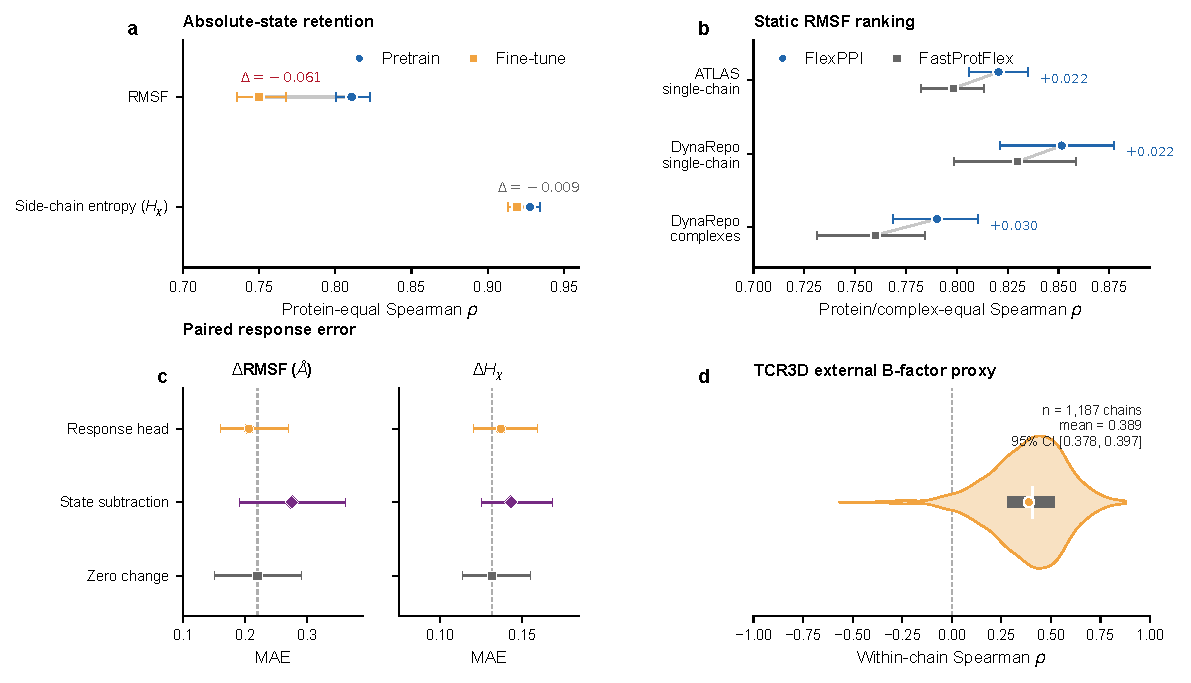
\includegraphics[width=\textwidth]{fig_completed_experiments.pdf}
  \caption{已完成柔性实验的统一可视化。所有点估计均先在单个蛋白、复合物或体系
  内计算，再对体系等权平均；误差线为归档结果中的非参数 bootstrap 95\% 置信
  区间。（a）预训练与配对响应微调后的绝对状态预测能力，仅展示 RMSF 与侧链
  构象熵 $H_\chi$，差值定义为微调减预训练。（b）FlexPPI 与 FastProtFlex
  在共同可回答的静态 RMSF 排序任务上的比较，右侧数字为
  $\rho_{\mathrm{FlexPPI}}-\rho_{\mathrm{FastProtFlex}}$。（c）7 个配对体系上
  响应头、状态相减和零变化基线的体系等权 MAE；竖虚线对应零变化基线，误差线
  反映当前小样本下的不确定性。（d）TCR3D 中 1,187 条可计算相关性的链的
  B-factor 代理 Spearman 分布；橙色点为链等权均值，灰色线为其 95\% 置信
  区间。TCR3D 共评测 1,189 条链，其中 2 条因代理值或预测值为常数而不能计算
  Spearman。面板（a）--（c）属于内部验证或模型选择诊断，面板（d）使用晶体
  B-factor 代理而非 MD 真值，因而均不作为独立测试集上的最终性能声明。}
  \label{fig:completed-experiments}
\end{figure}
\clearpage

\subsection{必须补做：冻结的外部柔性测试}

正式柔性结论需要建立完全未参与训练、调参和 checkpoint 选择的外部 MD 测试集。
候选体系在进入测试前必须同时与全部训练链进行 MMseqs2 序列搜索以及
Foldseek/CATH/ECOD 结构拓扑搜索，至少剔除高于 30\% 序列一致性的近同源，
并分别报告 ``新序列但旧折叠'' 和 ``新折叠''。每个体系应包含不少于三条独立
初速度的重复轨迹，在统一温度、力场、水模型、离子条件、平衡流程和生产时长下
生成标签；重复 A 对重复 B 的性能作为经验噪声上限。所有方法统一使用
$C_\alpha$、链级 Kabsch 对齐、共同残基掩码和缺失残基规则。

第一轮必须运行常数、氨基酸类型、二级结构、SASA、反向 pLDDT、GNM、ANM、
CABS-flex、FastProtFlex、FlexPred-SVR、PEGASUS、Flexpert-Seq 和
Flexpert-3D。第二轮加入 BackFlip、RocketSHP 和 RMSF-net 的 PDB-only 分支。
绝对输出模型参加 MAE/RMSE/CCC；相对输出模型只参加每蛋白相关、排序和
top-$k$ 检出。BackFlip 的局部对齐标签与 FlexPPI 的链级对齐标签分开报告，
RMSF-net 完整 cryo-EM 模型进入额外实验信息轨道。

\subsection{必须补做：独立 apo/holo 响应测试}

需要重新冻结一套从未进入响应微调和轮次选择的 apo/holo 测试集，并补齐两态
RMSF、侧链熵和 SASA 标签。界面定义从当前的跨链
$C_\alpha\leq8\,\text{\AA}$ 升级为任意重原子
$\leq5\,\text{\AA}$，另设 $5$--$12\,\text{\AA}$ 近界面和远端变构区域。
响应头、状态相减和零变化三种方法并列；每种训练至少使用五个随机种子，报告
蛋白级 bootstrap 区间、配对显著性检验、方向 macro-F1、强变化 AP、推理时间
和失败样本。还需比较冻结编码器、顶部小学习率解冻、旧任务 replay 和多任务
checkpoint 选择，以确定哪种方案能在学习响应时保留绝对状态能力。

\subsection{计划实验：由柔性响应预测结合亲和力}

亲和力实验分成两个任务。任务一预测复合物的
$\Delta G_{\mathrm{bind}}^{\circ}$；任务二预测突变或条件变化造成的
$\Delta\Delta G$。所有 $K_d/K_i$ 标签转换为统一的
$\mathrm{kcal\,mol^{-1}}$，保存温度、pH、离子强度、测量方法和不等式标签；
无法确定温度的样本单列或使用带缺失条件的模型，不能静默假设所有实验等价。
数据划分以复合物家族和界面相似性为单位，任何相同或近同源链、相同界面模板
及同一突变的正反记录不得跨越训练、验证和测试。

对每个样本按式 \eqref{eq:two-sided-response} 生成 A、B 双侧特征。主模型使用
式 \eqref{eq:symmetric-pooling} 的 A/B 对称表示；第一阶段冻结 FlexPPI，
只训练亲和力头，第二阶段小学习率解冻顶部表示块并保留
$\mathcal L_{\mathrm{pair}}$。主指标为复合物等权 MAE、RMSE、Pearson、
Spearman、$R^2$、CCC 和预测区间覆盖率；$\Delta\Delta G$ 另外报告稳定化/
去稳定化方向准确率、macro-F1 和反向反对称误差。

亲和力消融至少包含：（1）仅静态界面几何与理化特征；（2）仅绝对 RMSF、
侧链熵和 SASA；（3）仅直接柔性响应；（4）仅状态相减；（5）仅残基隐藏表示；
（6）静态与动态全部特征；（7）逐一移除 RMSF、侧链熵或 SASA；（8）真实
apo/holo 与从复合体删除伙伴的伪 apo 对照；（9）预训练状态 checkpoint、
响应微调 checkpoint 和带 replay 的联合 checkpoint。只有当 ``静态+动态''
在冻结同源/界面测试集上稳定超过 ``仅静态''，且多个随机种子的改进置信区间
不跨零，才能声称柔性响应为亲和力预测提供了增量价值。
